% domain of integration for whole-atom scattering
\begin{center}
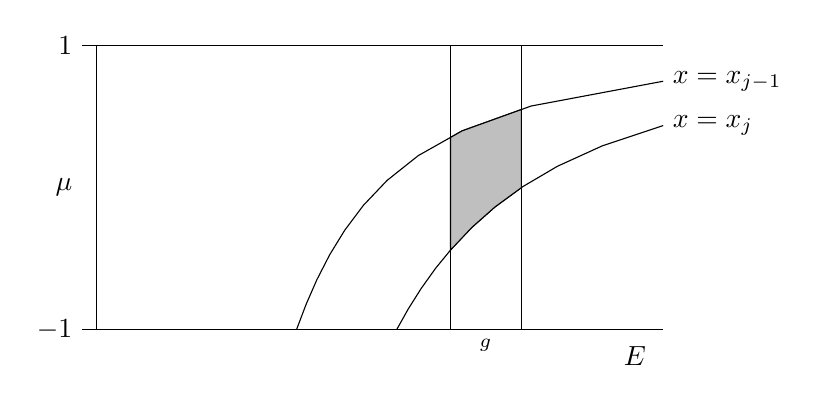
\begin{tikzpicture} [scale=1.8]
% the axes and quadrature box
  \draw(-0.1, -1) -- (4, -1);
  \draw(0, -1) -- (0, 1);
  \draw(-0.1, 1) -- (4, 1);
  \draw(2.5, -1) -- (2.5, 1);
  \draw(3, -1) -- (3, 1);
% x = constant curves
% E' = 2/sqrt{1 - mu}
\draw( 1.4142 , -1.0 ) --
( 1.4805 , -0.825 ) --
( 1.5570, -0.65 ) --
( 1.6468 , -0.475 ) --
( 1.7541, -0.3 ) --
( 1.8856, -0.125 ) --
( 2.0520, 0.05 ) --
( 2.2718, 0.225 ) --
( 2.5820, 0.4 ) --
( 3.0679, 0.575 ) --
( 4.0 , 0.75 );
% E' = 3/sqrt{1 - mu}
\draw( 2.1213, -1.0 ) --
( 2.2019, -0.85625 ) --
( 2.2925, -0.7125 ) --
( 2.3952, -0.56875 ) --
( 2.5131, -0.425 ) --
( 2.6504, -0.28125 ) --
( 2.8128, -0.1375 ) --
( 3.0094 , 0.00625 ) --
( 3.2540, 0.15 ) --
( 3.5698, 0.2938 ) --
( 4.0 , 0.4375 );
% integration region
\filldraw[fill = gray!50] (2.5000, -0.4410) --
( 2.6504, -0.28125 ) --
( 2.8128, -0.1375 ) --
(3.0000, -0.0006) --
(3.0000, 0.5505) --
( 2.5820, 0.4 ) --
( 2.5000, 0.3537) -- cycle;
% labels
  \node[left] at(-0.1, -1){$-1$};
  \node[left]  at(-0.1, 1){$1$};
  \node[left]  at(-0.1, 0){$\mu$};
  \node[below] at(2.75, -1){$\calE_g$};
  \node[below]  at(3.8, -1.05){$E$};
  \node[right] at(4, 0.75){$x = x_{j-1}$};
  \node[right]  at(4, 0.4375){$x = x_j$};
\end{tikzpicture}
\caption{Domain of integration for whole-atom scattering}
\label{Fig:coherent}
\end{center} 
